% This file is for creating and tweaking one plot at a time. When working on one plot, we don't want
% to do that in the context of a document that contains a lot of other stuff because that makes the
% edit -> compile -> inspect cycle very long. We create and tweak the plot here and once it's
% finished, we move the code over into another place like DemoPlots.tex.

%\documentclass[12pt, twocolumn]{article}
%\documentclass[12pt, openany]{book}
\documentclass[12pt, oneside]{book}
%\usepackage{fullpage}           % makes all margins 1 inch?
\topmargin=-1.0cm
\textheight=23cm
\evensidemargin=-1.0cm
\oddsidemargin=-1.0cm
\textwidth=19cm
\setcounter{secnumdepth}{-1}  % suppress numbering of sections
\usepackage{amsmath}
\usepackage{amssymb}          % for mathbb
\usepackage{hyperref}
\usepackage{array}            % For Cayley tables
\usepackage{stmaryrd}         % for \llbracket, \rrbracket
%\usepackage{cancel}           % \cancel to strike out math symbols - nah - it's ugly

\usepackage{comment}          
% to comment out larger sections via \begin{comment} ... \end{comment} 
% see:
% https://tex.stackexchange.com/questions/17816/commenting-out-large-sections
% https://tex.stackexchange.com/questions/11177/how-to-write-hidden-notes-in-a-latex-file/73418


\usepackage{color}               % colored text
\usepackage{listings}            % source code formatting 
%\lstset{language=python}
\definecolor{mygreen}{rgb}{0,0.6,0}
\definecolor{mygray}{rgb}{0.5,0.5,0.5}
\definecolor{mymauve}{rgb}{0.58,0,0.82}
\lstset{ %
  backgroundcolor=\color{white},   
  %basicstyle=\footnotesize\ttfamily,  % the size of the fonts that are used for the code
  basicstyle=\ttfamily,               % the size of the fonts that are used for the code
  captionpos=none,                    % no captions (and no empty space either)
  commentstyle=\color{mygreen},       % comment style
  frame=single,	                      % adds a frame around the code
  keywordstyle=\color{blue},          % keyword style
  language=Python,
  stringstyle=\color{mymauve},        % string literal style
  columns=flexible,                   %
  keepspaces=true,                    % keeps spaces in text
  tabsize=4,
}


\usepackage{tikz}
%\usetikzlibrary{calc} % maybe later
\usetikzlibrary{positioning}


\usepackage{mathtools}                        % for "\DeclarePairedDelimiter" macro

% Constants:
\DeclareMathOperator{\e}{\mathrm{e}}          % for Euler's number - ToDo: use \e consistently!
%\newcommand{\e}{\operatorname{e}}            % ...alternative definition (possibly)

% Functions:
\DeclareMathOperator{\li}{li}                      % Integral logarithm
\DeclareMathOperator{\Li}{Li}                      % Integral logarithm
\DeclareMathOperator{\sign}{sign}    
\DeclareMathOperator{\atan2}{atan2}
\DeclarePairedDelimiter{\floor}{\lfloor}{\rfloor}
\newcommand{\norm}[1]{\left\lVert#1\right\rVert}   % different norms?

% Matrix stuff:
\DeclareMathOperator{\rank}{rank}             % rank
\DeclareMathOperator{\vectorize}{vec}         % matrix to vector (concat columns)
\DeclareMathOperator{\tr}{tr}                 % trace
\DeclareMathOperator{\geo}{geo}               % geometric multiplicity
\DeclareMathOperator{\alg}{alg}               % algebraic multiplicity 

% Multivariable calculus:
%\DeclareMathOperator{\d}{d}                  % exterior derivative
\DeclareMathOperator{\grad}{\mathbf{grad}}
\DeclareMathOperator{\curl}{\mathbf{curl}}
\DeclareMathOperator{\dive}{div}

% Set theory:
\DeclareMathOperator{\im}{im}                 % image of a function/map
\DeclareMathOperator{\card}{card}             % cardinality        
\DeclareMathOperator{\tc}{tc}                 % transitive closure of a set
%\DeclareMathOperator{\Eig}{Eig} 

% Logic:
% There are multiple conventions to express a logical exclusive or - we make the choice for the
% whole text here:
\newcommand*\xor{\mathbin{\veebar}}              % exclusive or - alternatives: \oplus, \dot{\vee}
\newcommand*\nand{\mathbin{\barwedge}}
\newcommand*\then{\mathbin{\rightarrow}}         % \implies is already defined
\newcommand*\mequiv{\mathbin{\leftrightarrow}}   % material equivalence
% We follow wolfram:
% https://mathworld.wolfram.com/XOR.html
% https://mathworld.wolfram.com/NAND.html

%\let\cleardoublepage\clearpage

% Maybe move the stuff up to here into a _Setup.tex file that can be included from
% _FullBook.tex and _SingleChapter.tex



\begin{document}


\begin{figure}[h]
\centering
\pgfplotsset{width=18cm,height=12cm} 
\pgfplotsset{compat=1.9}

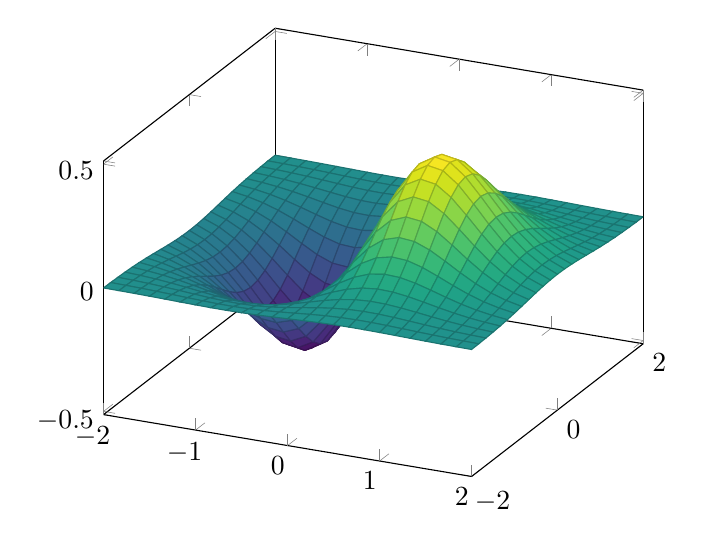
\begin{tikzpicture}
\begin{axis}%[title=Bivariate Gaussian]
   \addplot3 [surf,colormap/viridis,domain=-2:2] {x * exp(-x^2-y^2)};
\end{axis}
\end{tikzpicture}


% Try using "colormap/viridis" instead of "fill=white"
% ...done - yes - looks better - but maybe use more samples - it looks a bit rough
\end{figure}


%---------------------------------------------------------------------------------------------------
% 3D plots with arrows drawn in


\pgfplotsset{width=16cm,height=10cm,compat=1.12}
\begin{tikzpicture}[thick, >=stealth']
\begin{axis}[xlabel={$x$}, ylabel={$y$}, xmin=-1.5,xmax=1.5,ymin=-1.5,ymax=+1.5, samples=17]
  \addplot3[surf, faceted color=black, fill=white, domain=-1:1, y domain=-1:1] 
  {1-x^2-y^2};
%  \draw[->, ultra thick] (0,0,0) -- (1,1,0);
%  \fill[red] (0.5,-0.25,0.625) circle (3pt);
\fill[red] (0.5,-0.5,0.5) circle (3pt);
\end{axis}
\end{tikzpicture}
% "domain" means "x domain", "y domain" means what it says
% surf does not seem to accept the draw=black command - ah one needs to use "faceted color = black"


\pgfplotsset{width=16cm,height=10cm,compat=1.12}
\begin{tikzpicture}[thick, >=stealth']
\begin{axis}[xlabel={$x$}, ylabel={$y$}, xmin=-2,xmax=2,ymin=-2,ymax=+2,samples=11]
  \addplot3[surf, mesh, color=gray, domain=-1:1, y domain = -1:1] {x+y+1};
  %\draw[->, thick, red]   (0,0,0) -- (1,0,0);
  %\draw[->, thick, green] (0,0,0) -- (0,1,0);
  %\draw[->, thick, blue]  (0,0,0) -- (0,0,1);
  \draw[->, ultra thick] (0,0,0) -- (1,1,0);
  \fill[black] (0,0,0) circle (3pt);
\end{axis}
\end{tikzpicture}


% trying to draw in 3D arrows
% https://tex.stackexchange.com/questions/267222/3d-arrows-with-tikz
% shows also how to set local variables (using pgfsetmacro)

% This looks relevant:
% https://tex.stackexchange.com/questions/310478/pgfplot-3d-version-of-a-plane-and-its-the-gradient-vector

\pgfplotsset{width=16cm,height=10cm,compat=1.12}
\begin{tikzpicture}[thick, >=stealth']
\begin{axis}[xlabel={$x$}, ylabel={$y$}]
  \addplot3[surf, mesh] {x+y+1};
  \draw[->, ultra thick] (0,0,0) -- (1,1,0);
  \fill[black] (0,0,0) circle (3pt);
\end{axis}
\end{tikzpicture}
% It's important to use compat=1.12 ...or maybe higher. With 1.9, it didn't work
% ToDo: the arrow-head still looks kinda ugly - try to improve that - ok - done


% See also:
% https://tex.stackexchange.com/questions/518504/how-can-i-draw-gradient-arrows-on-iso-contour
% https://tex.stackexchange.com/questions/631435/tikz-3d-surface-plot

% Try drawing a torus with tangential plane, unit normal vector - or maybe have multiple normal 
%  vectors sticking out
% https://tex.stackexchange.com/questions/348/how-to-draw-a-torus
% https://latexdraw.com/how-to-draw-a-torus-in-latex-using-tikz/?utm_content=cmp-true#t-1608582125077
% https://tikz.net/torus/

\end{document}